\section{Cookies}
Cookies werden f�r die Identifizierung des Surfers genutzt. Neben der erw�nschten Identifizierung um personalisierte Inhalte zu nutzen, beispielsweise einen Web-Mail-Account oder um Eink�ufe abzuwickeln, werden sie auch f�r das Tracking von Nutzern verwendet.\\

Der Screenshot Bild \ref{abb:cookiespiegel} zeigt die Liste der Cookies, die bei einem einmaligen Aufruf der Seite \textit{www.spiegel.de} gesetzt wurden. Neben den Cookies von \textit{spiegel.de} zur Z�hlung der Leser setzen gleich mehrere datensammelnde Werbeserver Cookies und au�erdem Z�hldienste (quality-chanel.de, ivwbox.de), welche die Reichweiten von Online-Publikationen auswerten.\\

\begin{figure}[p]
\begin{center}
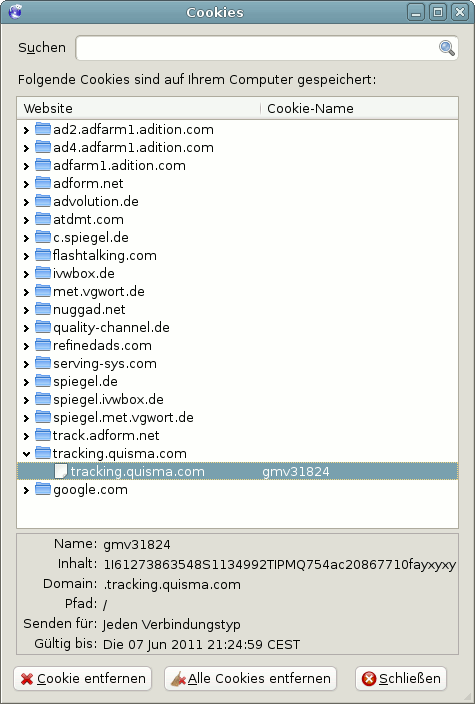
\includegraphics[scale=0.75]{../screenshots/cookies_spiegel.png}
\caption{Liste der Cookies beim Besuch von Spiegel-Online}
\label{abb:cookiespiegel}
\end{center}
\end{figure}

Es ist nicht ungew�hnlich, dass popul�re Webseiten mehrere Datensammler einbinden. Eine Studie der Universit�t Berkeley \footnote{ \href{http://heise.de/-1288914}{http://heise.de/-1288914}}  hat 2011 beim Surfen auf den TOP100 Webseiten 5.675 Cookies gefunden (ohne Login oder Bestellung). 4.914 Cookies wurden von Dritten gesetzt, also nicht von der aufgerufenen Webseite. Die Daten wurden an mehr als 600 Server �bermittelt. Spitzenreiter unter den Datensammlern ist Google, 97\% der popul�ren Webseiten setzen Google-Cookies.\\

Sinnvoll ist ein \textbf{Whitelisting} f�r die Behandlung von Cookies:

\begin{enumerate}
\item Standardm��ig wird die Annahme von Cookies verweigert.
\item F�r vertrauensw�rdige Websites, welche die Nutzung von Cookies zur Erreichung der vollen Funktion ben�tigen, werden Ausnahmen zugelassen.
\item Die f�r den Zugriff auf personalisierte Inhalte gespeicherten Cookies sollten beim Schlie�en des Browsers automatisch gel�scht werden. Einige Websites verwenden diese Cookies auch nach dem Logout f�r das User-Tracking.
\end{enumerate} 

Fast alle Login-Seiten, welche Cookies zur Identifizierung des Surfers verwenden, weisen mit einem kleinen Satz auf die notwendigen Freigaben hin. Treten beim Login seltsame Fehler auf, z.B. st�ndig die Fehlermeldung \textit{FALSCHES PASSWORT}, verweigert der Browser wahrscheinlich die Annahme von Cookies. Die Website sollte in die Liste der vertrauensw�rdigen Websites aufgenommen werden.\\


